\chapter{Inferring the Causes of Real-World Rogue Waves} \label{chap:main}

\sidefigure{AI art generated by VQGAN + CLIP \citep{esser_taming_2021,radford_learning_2021}. Prompt: \emph{\enquote{offshore oil platform in a storm | rogue wave | illustration}}.}{
    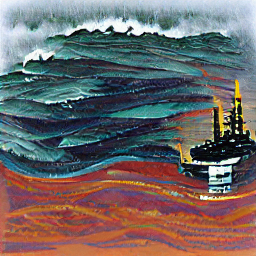
\includegraphics[width=.9\linewidth]{vqgan-images/vqgan-6.png}
}
%
The overarching goal of this thesis is to infer the causes of measured oceanic rogue waves from data.
This could provide some much needed evidence to the field, because there are several plausible hypotheses on the generation mechanisms of rogue waves, but no consensus regarding which ones are dominant in the ocean and where to put the main research focus (see \secref{sec:sota-rogue}).

The central idea to tackle this is to infer how rogue wave occurrence depends on the sea state (\ie, which parameters govern rogue wave generation). We can then tie this back to a generation mechanism by interpreting the identified dependencies in light of the comprehensive corpus of theoretical literature.

To perform this inference we use \enquote{black box} machine learning methods such as deep neural networks and random forest classifiers, in connection with more traditional Bayesian methods and a causal analysis. The immense success of machine learning has often falsely led it to be considered a silver bullet that can and should be applied to any data problem, even though traditional statistics and data analysis methods may offer better or more interpretable results. But in the case of rogue waves, modern machine learning is able to handle a unique set of challenges that traditional methods are not equipped to tackle.

\marginelement{
    Algorithmic requirements to study probabilistic extreme events:\\[\baselineskip]
    \begin{marginenum}
        \item Scales to massive amounts of data;
        \item Quantifies uncertainty;
        \item Captures nonlinearity and interactions.
    \end{marginenum}
}
%
Rogue waves are exceedingly rare events, so we must collect and process massive amounts of data. Also, rogue waves may occur with a non-zero probability in any condition (\ie the classes \enquote{rogue seas} and \enquote{non-rogue seas} are not separable). This means that we cannot discard non-events, and only relative event rates --- \emph{rogue wave probabilities} --- are meaningful. To make things worse, the fact that they are rare events forces us to carefully consider the effects of limited data volumes. This makes for an enormously challenging task for learning algorithms: They need to scale to \emph{big data} while providing uncertainty quantification and robustness that is mostly used in the context of \emph{little data} --- and typically computationally expensive, \eg when using Bayesian methods based on sampling from a posterior distribution. At the same time, there is no universally accepted parametric form on how rogue wave probabilities depend on the sea state (or even which parameters are sufficient to fully characterize a sea state). This means that any chosen method will have to be \emph{flexible}, ideally supporting arbitrary nonlinear connections between parameters. Scaling and flexibility are inherent strengths of machine learning, and many methods can be augmented to quantify uncertainties. This makes them an excellent fit for this task.

\clearpage
The full objectives of this study are:
\marginelement{\spacedlowsmallcaps{Objectives}}

\begin{renum}
    \item Assemble a dataset that contains enough data to study rogue waves throughout a wide regime of sea states.
    \item Explore the unique challenges in large-scale wave data curation for machine learning applications (since this is the first study at this scale).
    \item Analyze how rogue wave occurrence depends on sea state parameters, taking uncertainties due to limited data into account.
    \item Determine whether there are sea states of significantly higher rogue wave risk (which could settle the question whether rogue waves are rare realizations of common sea states or common realizations of rare sea states).
    \item Infer the dominant creation mechanisms of rogue waves.
    \item Suggest a way forward for rogue wave \emph{prediction}.
\end{renum}

The central part of this thesis consists of 3 research articles that address all of these issues.

\cleardoublepage
\section{Article I --- FOWD: A Free Ocean Wave Dataset for Data Mining and Machine Learning}

\begin{figure}
    \strictpagechecktrue
    \begin{sidecaption}{The locations of all CDIP buoys. Most buoys are located in relatively shallow water off the Southern Californian coast, but some deep water buoys with long time records exist (\eg around Hawaii). Based on the CDIP station map at \href{https://cdip.ucsd.edu}{\texttt{cdip.ucsd.edu}}.}[fig:cdip]
    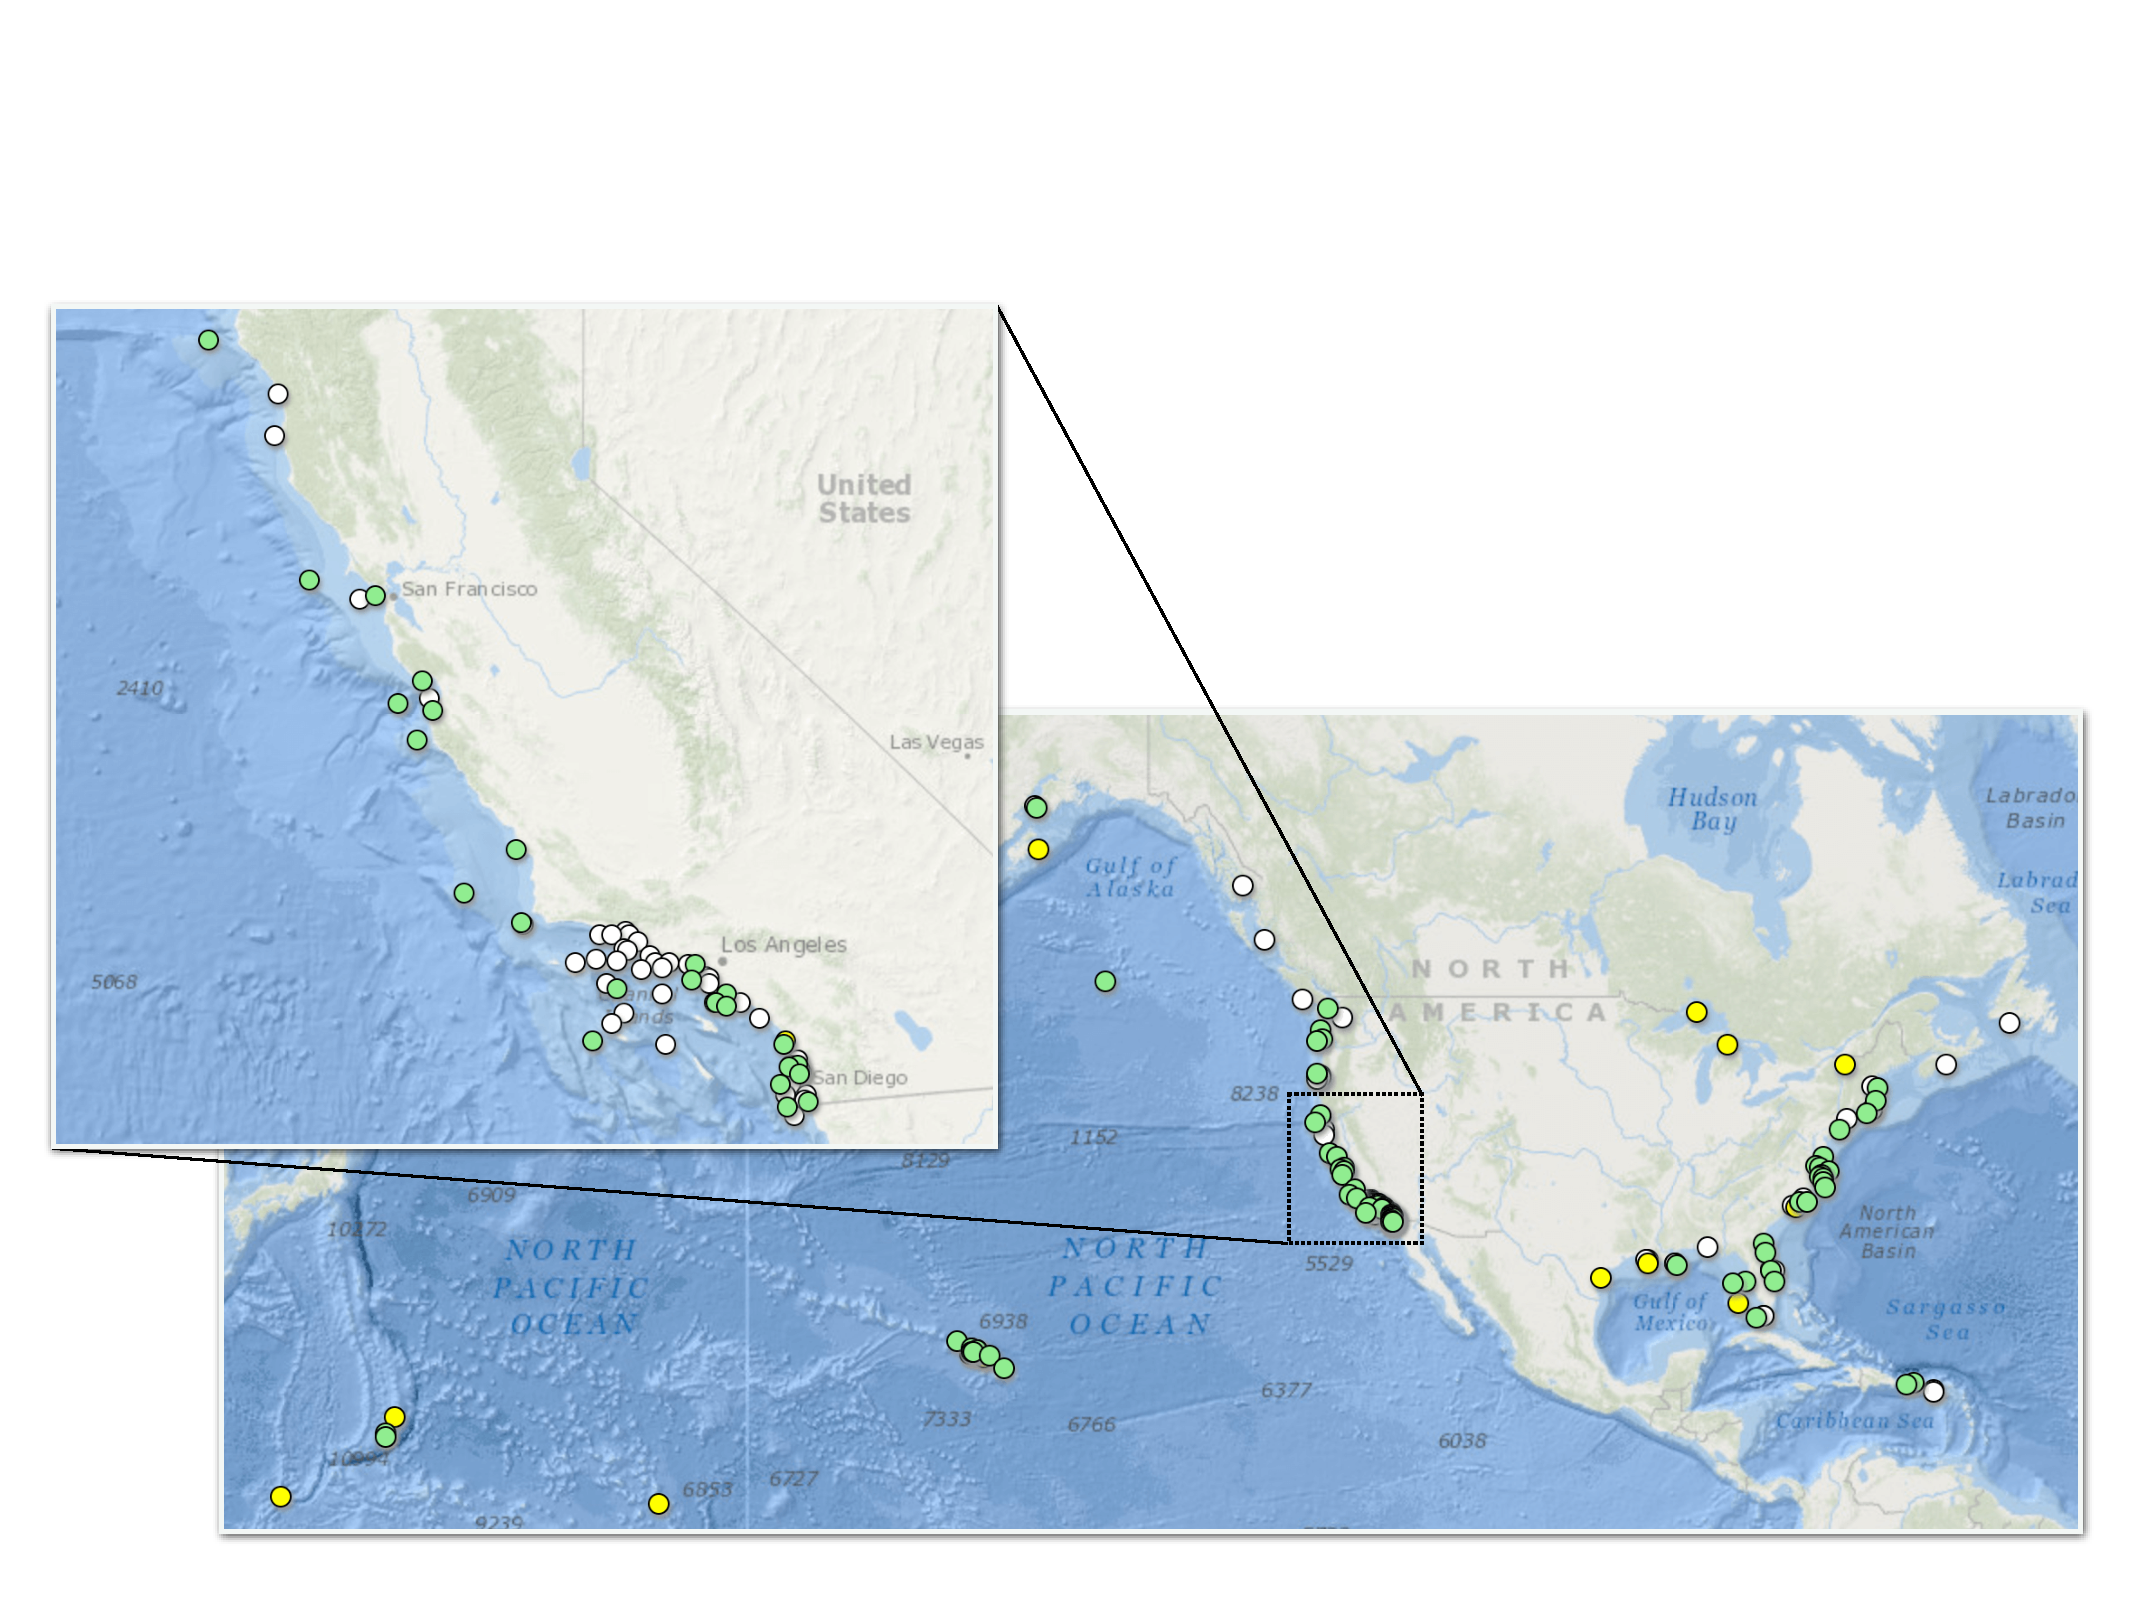
\includegraphics[width=\linewidth,trim=8mm 8mm 8mm 48mm,clip]{main/fowd-station-map.pdf}
    \end{sidecaption}
\end{figure}

\sidefigure{AI art generated by VQGAN + CLIP \citep{esser_taming_2021,radford_learning_2021}. Prompt: \emph{\enquote{rogue wave book cover}}.}{
    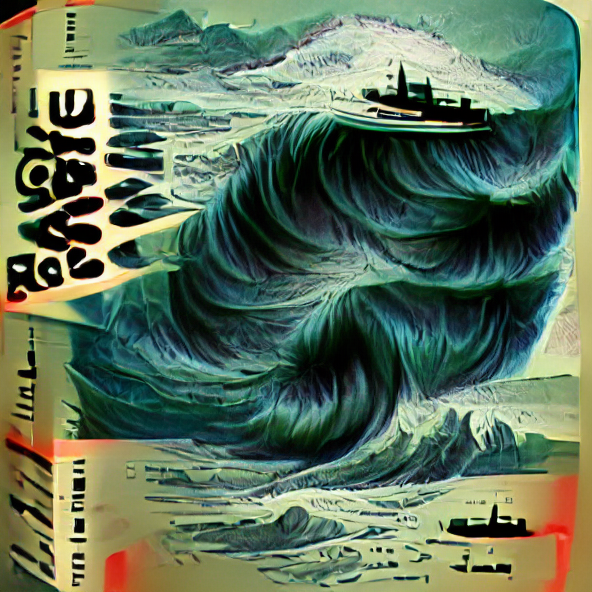
\includegraphics[width=.9\linewidth]{vqgan-images/vqgan-40.png}
}
%
This first article \citep{hafner_fowd_2021} serves as the foundation of all further work by assembling a large catalogue of waves and sea states that we call FOWD (Free Ocean Wave Dataset).

Since we need as much data as we can possibly get to study extreme wave statistics (which requires many thousands of rogue wave events), we decided to process the entire data catalogue of the Coastal Information Data Program \citep[CDIP,][]{behrens_cdip_2019}.
CDIP operates a network of more than 150 waverider buoys along the US coast and in US overseas territories (\figref{fig:cdip}), and supplies raw surface elevations in its outputs. This is a huge dataset --- some of these buoys have been measuring almost continuously since the 1990s at a sampling frequency of \SI{1.28}{\hertz}, which leads to a combined time series length of over 700 years.

We were also concerned that the usual approach of splitting the time series into equal-time chunks and observed maximum wave height \citep[as \eg in][]{casasprat_short-term_2010,christou_field_2014} would not be appropriate for machine learning, because the presence of a rogue wave biases sea state parameters that are sensitive to outliers and leads to confounding (where label information leaks into parameter space)\sidenote{As it turns out, rightfully so --- see our findings on surface elevation kurtosis in article 2.}. Therefore, we process the history of every wave in the record separately (over 4 billion waves total) with a running window (\figref{fig:fowd-workflow}).

\begin{figure}
    \strictpagechecktrue
    \begin{whole}
        \vspace*{-2.2cm}
        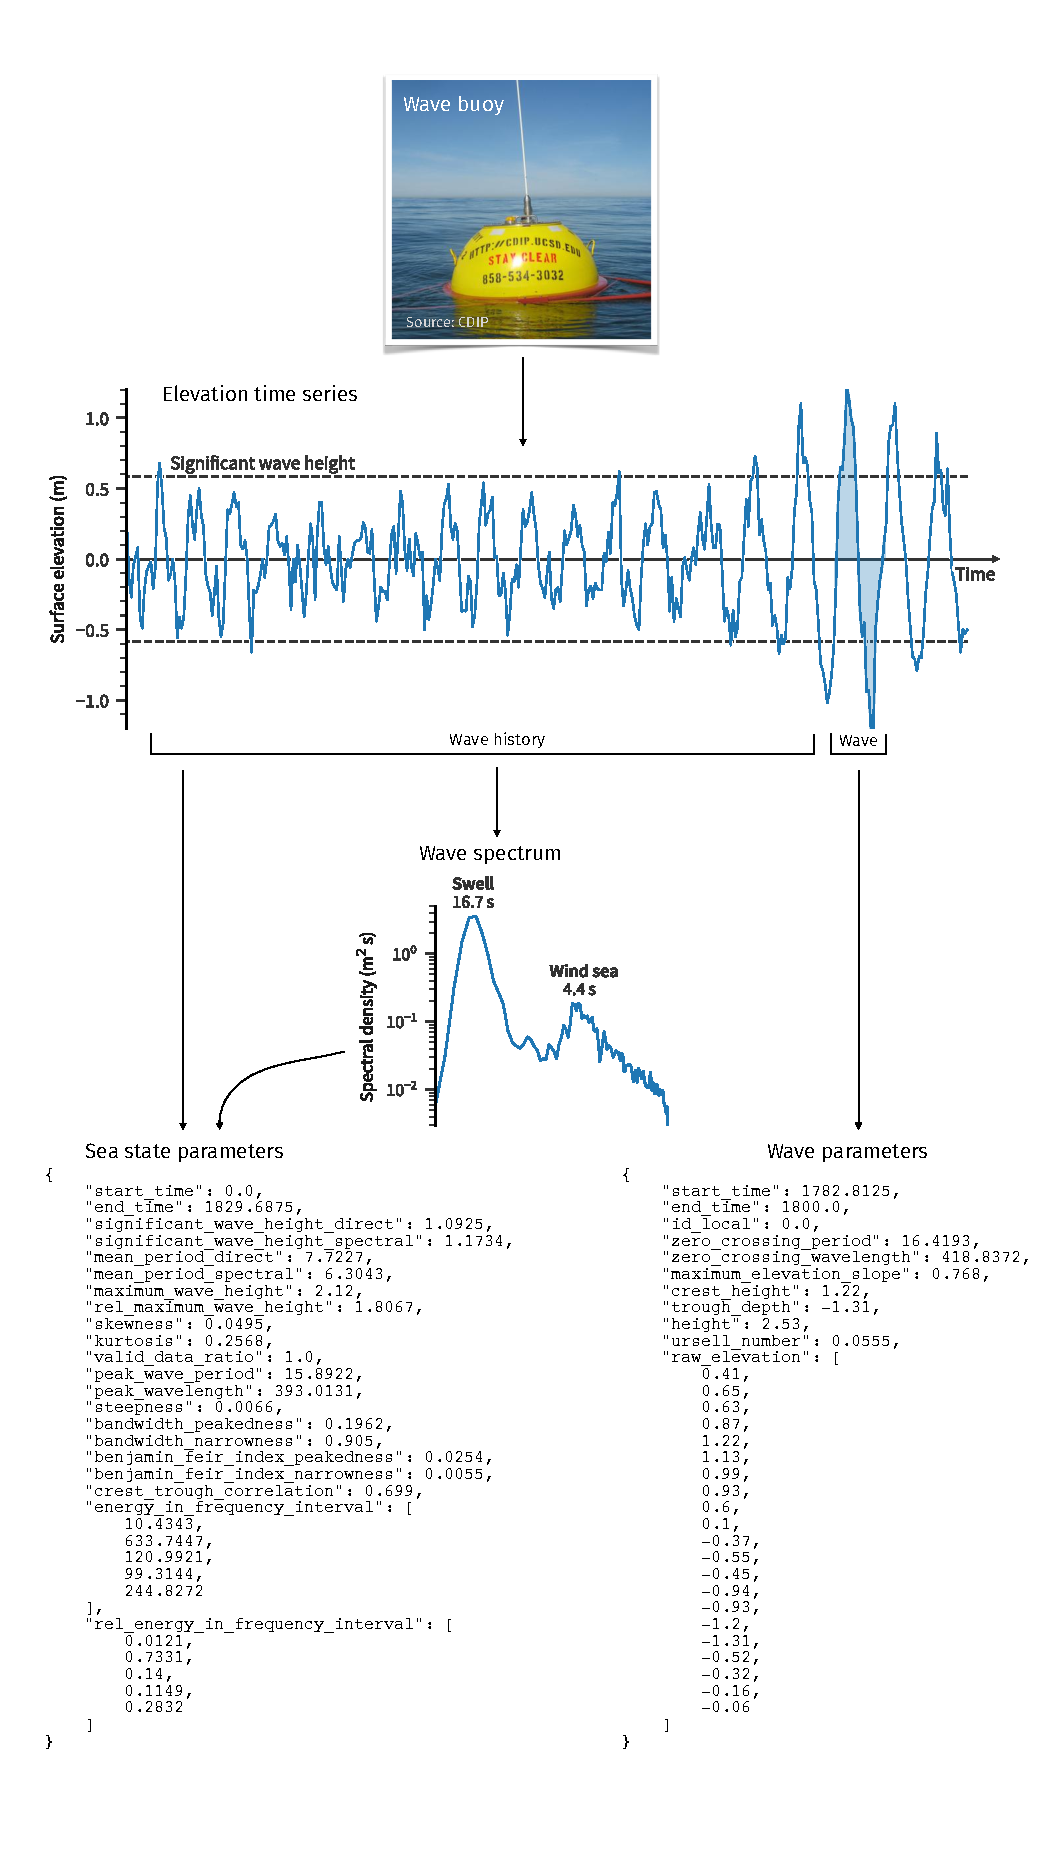
\includegraphics[width=.8\linewidth,trim=2mm 16mm 0mm 12mm,clip]{main/fowd-workflow-portrait.pdf}
    \end{whole}
    \caption{A real example of how FOWD processes a wave record, here containing a rogue wave ($H/H_s = 2.16$) in a swell-dominated sea. Sea state and wave parameters are computed for every zero-crossing wave in the measured elevation time series with a running window.} \label{fig:fowd-workflow}
\end{figure}

As we have to process billions of sea states, this approach comes with a considerable computational demand. We solve this through a memory-efficient implementation that allows us to process many stations in parallel. The final output dataset is about \SI{1}{\tera\byte} in size and freely available for download.

To get a first idea of how rogue waves depend on the sea state, we need to find how the rogue wave probability $p$ varies with each sea state parameter. We also want to achieve this without assuming a functional dependency of $p$ on the parameters (this rules out something like logistic regression which assumes a linear connection), and quantify uncertainties in our estimates.

This led us to develop \enquote{Bayesian histograms}\sidenote{A Python package for Bayesian histograms is now available at \href{https://github.com/dionhaefner/bayesian-histograms/}{\path{github.com/dionhaefner/bayesian-histograms}}.}, where we apply a binning to each parameter and assume that $p$ is identically, independently Beta-distributed within each bin (\ie that rogue and non-rogue samples within each bin are drawn randomly with a constant rogue wave probability $p$). Choosing an appropriate conjugate prior for $p$, this gives us a non-parametric way to estimate $p$ and its uncertainty depending on each parameter without expensive Monte Carlo sampling (\figref{fig:bayeshist}).

When applying Bayesian histograms to a subset of FOWD, we find that spectral bandwidth, crest-trough correlation, and surface elevation kurtosis are most informative (cause the biggest variation in $p$) --- a result that is revisited and studied in much more detail in article 2.

\begin{figure}[b]
    \caption{An example of a Bayesian histogram on generated (fake) data. The Bayesian histogram estimate of the event rate (rogue wave probability) $p$ is based on the ratio between positive and negative samples within each bin. Uncertainties are higher in regions with less data and in regions with lower values of $p$.} \label{fig:bayeshist}
    \strictpagechecktrue
    \begin{whole}
    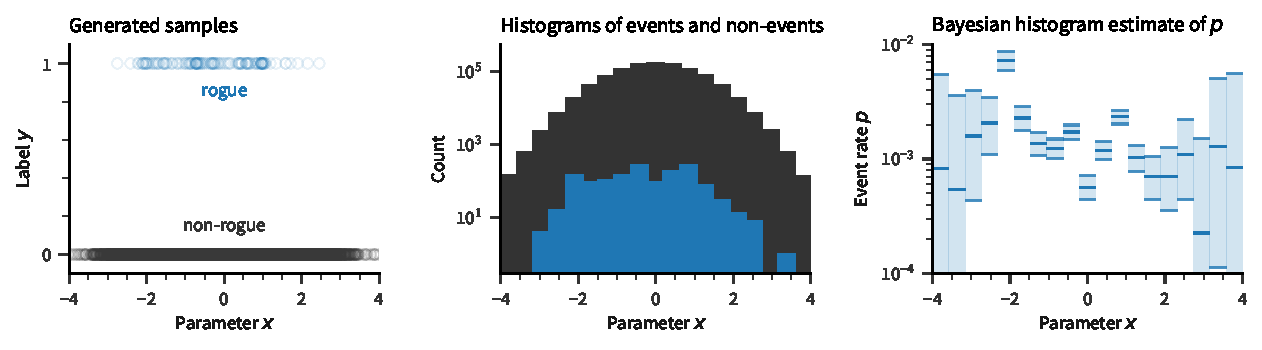
\includegraphics[width=\linewidth]{main/bayesian-histogram.pdf}
    \end{whole}
\end{figure}

\includepaper[trim=0mm 7.2mm 0mm 14mm,clip]{Article I --- FOWD: A Free Ocean Wave Dataset for Data Mining and Machine Learning}{papers/1-jtech.pdf}

\cleardoublepage
\section{Article II --- Real-world Rogue Wave Probabilities} \label{sec:rogueprob}

\sidefigure{AI art generated by VQGAN + CLIP \citep{esser_taming_2021,radford_learning_2021}. Prompt: \emph{\enquote{a ship hit by a rogue wave in the distance:80 | unsplash:20}}.}{
    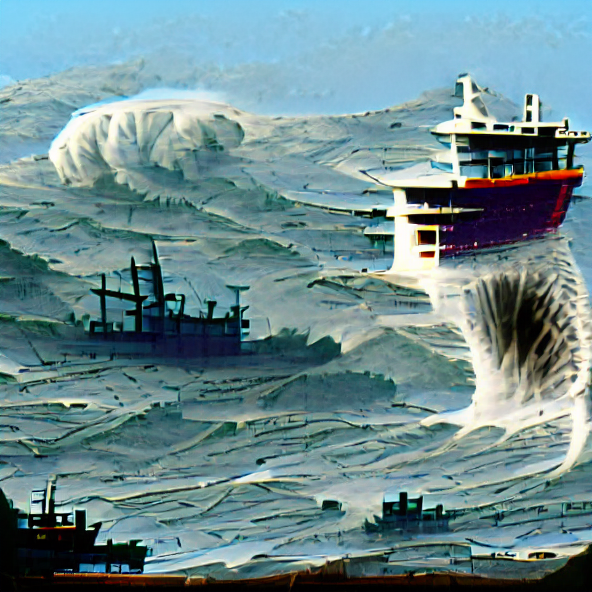
\includegraphics[width=.9\linewidth]{vqgan-images/vqgan-11.png}
}
%
Now that we have access to a large high-quality dataset, we can search for parameter combinations with significantly enhanced rogue wave activity. We address this in the second article \citep{hafner_real-world_2021}.

So far we have only looked at a subset of the full FOWD data, and at each parameter in isolation. To remedy the former we aggregate the FOWD dataset into chunks of 100 waves in which we assume the sea state to be constant, which allows us to analyze the entire dataset at once. We once again use Bayesian histograms for the univariate analysis. To control for correlations between parameters we study conditional probabilities through the same approach, which gives some first evidence on the causal structure of the problem (through observed conditional independencies). For this we introduce the quantity \emph{predictive power}, which measures by how much $p$ changes as each parameter is varied.

We also need to determine whether there are significant interactions between parameters (because if there are, a univariate analysis will be highly misleading), again in a non-parametric way and with uncertainties. There is no off-the-rack machine learning algorithm that fits these requirements considering our data volume and low event rates. This led us to develop our own method for this task.

For the multivariate analysis, we use a shallow decision tree surrogate model to cluster the rogue wave probability $p$ (estimated through a deep random forest classifier) into high-dimensional rectangular regions with approximately constant $p$ (\figref{fig:uncertain-forest}). We then interpret the results of this process separately for each cluster in the same way as in the univariate case, which also gives us uncertainties of $p$ within each cluster (based on unseen validation data to mitigate overfitting).

This approach, similar to Bayesian histograms, is quite conservative and not the strongest learner, since it assumes no dependence between neighboring bins / clusters whatsoever, but in our case we have enough data to be able to value robustness over exploitation. Our multivariate analysis shows that feature interactions are generally weak, so we focus on the univariate analysis in the article.

Our analysis reveals that crest-trough correlation is the dominant causal parameter behind rogue wave formation. Surface elevation kurtosis, which we found to be an important parameter in article 1, has no predictive quality in the aggregated data, which suggests that it can only indicate whether a rogue wave is already forming and cannot be used for forecasting.

\begin{figure}
    \strictpagechecktrue
    \begin{whole}
        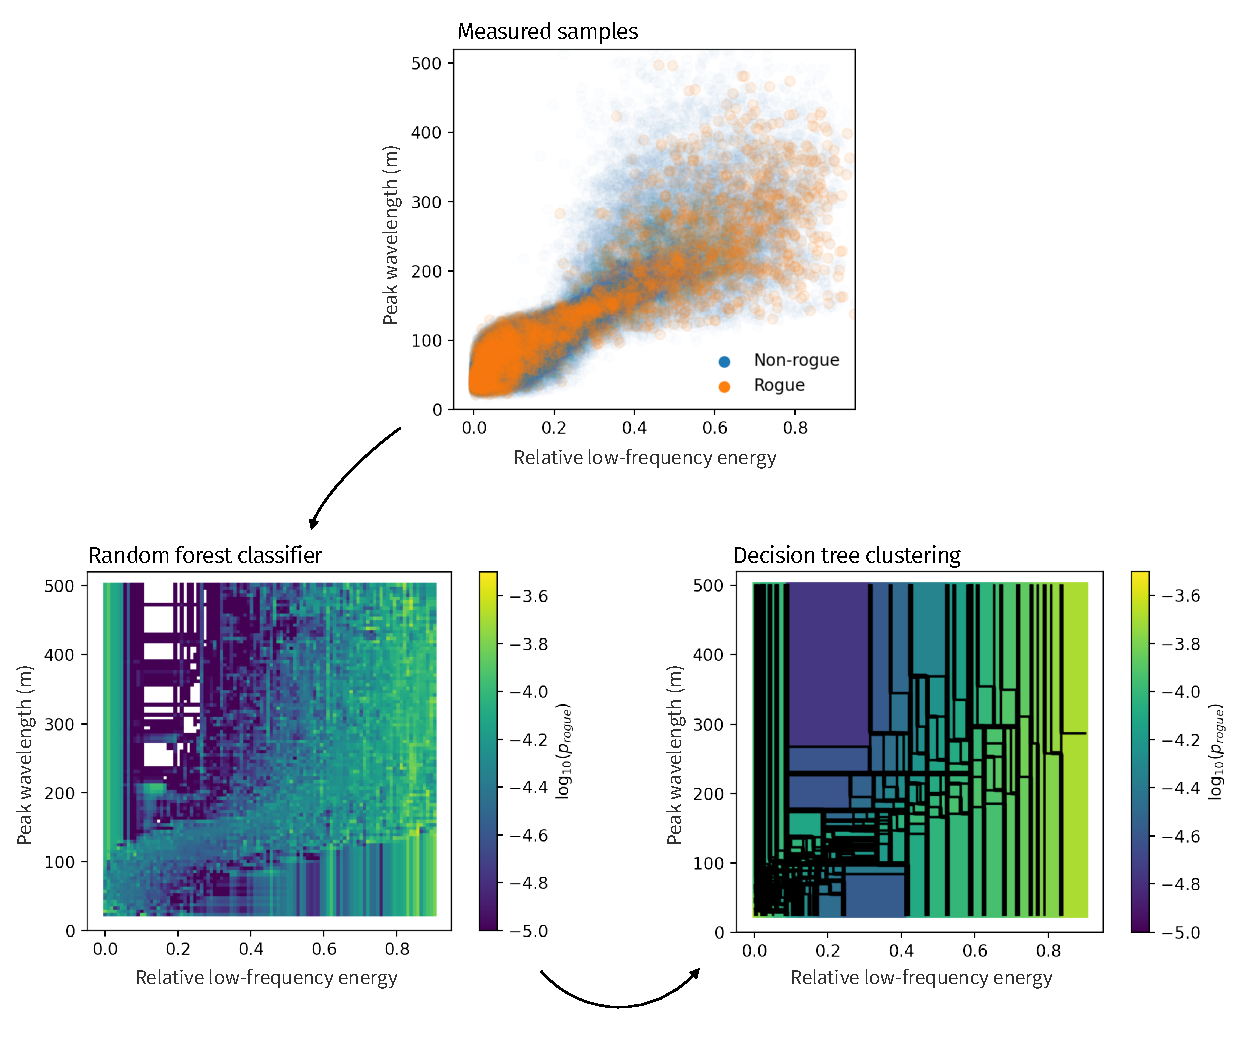
\includegraphics[width=\linewidth]{main/uncertain-forest.pdf}
    \end{whole}
    \caption{Decision tree clustering for rare events. In the first step, raw samples are converted into (noisy) probability estimates, \eg through a random forest classifier. In the second step, a surrogate decision tree model is trained on the output of the first model with (high) constant number of samples per leaf. The resulting leaves represent a rectangular partition in feature space where $p$ is approximately constant in each cluster. This allows us to analyze each cluster separately based on the number of rogue and non-rogue samples in it, just like in the univariate case.} \label{fig:uncertain-forest}
\end{figure}

\includepaper[trim=0mm 15mm 0mm 15mm,clip]{Article II --- Real-world Rogue Wave Probabilities}{papers/2-scirep.pdf}

\cleardoublepage
\section{Article III --- A Causal Predictive Model for Real-World Rogue Wave Probabilities} \label{sec:causalrogue}

\sidefigure{AI art generated by VQGAN + CLIP \citep{esser_taming_2021,radford_learning_2021}. Prompt: \emph{\enquote{the great wave}}.}{
    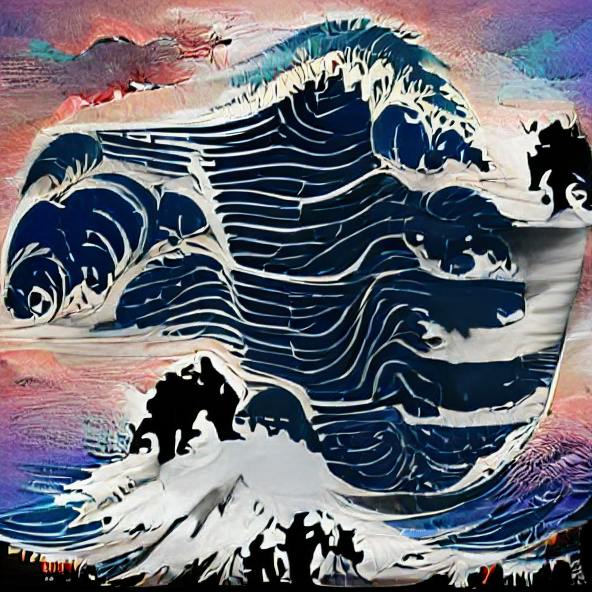
\includegraphics[width=.9\linewidth]{vqgan-images/vqgan-15.png}
}
%
The final article in this series (to be submitted) puts the previous findings on a more rigorous causal foundation, and demonstrates how we can use our results to arrive at a better rogue wave forecast.

For a well-performing predictive model we need to relax the assumption of independent regions in parameter space (as we used in the previous articles to study how the rogue wave probability $p$ depends on the sea state). Instead, we would now like to interpolate between data points through an artificial neural network, but this introduces a considerable risk of overfitting. To mitigate this, we perform a causal analysis based on the state-of-the-art in rogue wave research (as presented in \secref{sec:sota-rogue}) to include only \emph{direct causes} of rogue waves in the model. To limit the number of possible parameter interactions and combat overfitting we employ a multi-head neural network, where only parameters sharing the same input head can interact non-additively with each other.

To quantify how well the trained model captures the causal structure we apply a procedure that is inspired by invariant causal prediction \citep[ICP;][]{peters_causal_2016,peters_elements_2017}. We search for a model that stays approximately invariant under re-training on different environments (such as summer vs.\ winter conditions, or deep water vs.\ shallow water). This allows us to identify a model that represents a good trade-off between predictive performance and invariance.

Additionally, we visualize the prediction surface of this model and compare to the findings in article 2, which largely confirms earlier results, but also leads to some new insights on the nature of higher-order corrections due to parameter interactions. On top of this, we identify a crucial interaction between crest-trough correlation and directionality index that has (to our knowledge) not been described before.

\includepaper[trim=0mm 13mm 0mm 17mm,clip]{Article III --- A causal predictive model for real-world rogue wave probabilities (DRAFT)}{papers/3-causal-rogue-waves.pdf}
